\documentclass[a4paper,11pt]{article}
\usepackage{amsmath,amsthm,amsfonts,amssymb,amscd,amstext,vmargin,graphics,graphicx,tabularx,multicol} 
\usepackage[francais]{babel}
\usepackage[utf8]{inputenc}  
\usepackage[T1]{fontenc} 
\usepackage{pstricks-add,tikz,tkz-tab,variations}
\usepackage[autolanguage,np]{numprint} 
\usepackage{pifont}


\setmarginsrb{1.5cm}{0.5cm}{1cm}{0.5cm}{0cm}{0cm}{0cm}{0cm} %Gauche, haut, droite, haut
\newcounter{numexo}
\newcommand{\exo}[1]{\stepcounter{numexo}\noindent{\bf Exercice~\thenumexo} : \marginpar{\hfill /#1}}
\reversemarginpar


\newcounter{enumtabi}
\newcounter{enumtaba}
\newcommand{\q}{\stepcounter{enumtabi} \theenumtabi.  }
\newcommand{\qa}{\stepcounter{enumtaba} (\alph{enumtaba}) }
\newcommand{\initq}{\setcounter{enumtabi}{0}}
\newcommand{\initqa}{\setcounter{enumtaba}{0}}

\newcommand{\be}{\begin{enumerate}}
\newcommand{\ee}{\end{enumerate}}
\newcommand{\bi}{\begin{itemize}}
\newcommand{\ei}{\end{itemize}}
\newcommand{\bp}{\begin{pspicture*}}
\newcommand{\ep}{\end{pspicture*}}
\newcommand{\bt}{\begin{tabular}}
\newcommand{\et}{\end{tabular}}
\renewcommand{\tabularxcolumn}[1]{>{\centering}m{#1}} %(colonne m{} centrée, au lieu de p par défault) 
\newcommand{\tnl}{\tabularnewline}

\newcommand{\trait}{\noindent \rule{\linewidth}{0.2mm}}
\newcommand{\hs}[1]{\hspace{#1}}
\newcommand{\vs}[1]{\vspace{#1}}

\newcommand{\N}{\mathbb{N}}
\newcommand{\Z}{\mathbb{Z}}
\newcommand{\R}{\mathbb{R}}
\newcommand{\C}{\mathbb{C}}
\newcommand{\Dcal}{\mathcal{D}}
\newcommand{\Ccal}{\mathcal{C}}
\newcommand{\mc}{\mathcal}

\newcommand{\vect}[1]{\overrightarrow{#1}}
\newcommand{\ds}{\displaystyle}
\newcommand{\eq}{\quad \Leftrightarrow \quad}
\newcommand{\vecti}{\vec{\imath}}
\newcommand{\vectj}{\vec{\jmath}}
\newcommand{\Oij}{(O;\vec{\imath}, \vec{\jmath})}
\newcommand{\OIJ}{(O;I,J)}

\newcommand{\bmul}[1]{\begin{multicols}{#1}}
\newcommand{\emul}{\end{multicols}}

\newcommand{\reponse}[1][1]{%
\multido{}{#1}{\makebox[\linewidth]{\rule[0pt]{0pt}{20pt}\dotfill}
}}

\newcommand{\titre}[5] 
% #1: titre #2: haut gauche #3: bas gauche #4: haut droite #5: bas droite
{
\noindent #2 \hfill #4 \\
#3 \hfill #5

\vspace{-1.6cm}

\begin{center}\rule{6cm}{0.5mm}\end{center}
\vspace{0.2cm}
\begin{center}{\large{\textbf{#1}}}\end{center}
\begin{center}\rule{6cm}{0.5mm}\end{center}
}



\begin{document}
\pagestyle{empty}
\titre{Interrogation: Nombres relatifs}{Nom :}{Prénom :}{Classe}{Date}

\vspace*{0.2cm}






\exo{5} Calculer les expressions suivantes \textbf{en détaillant vos étapes de calcul}.\\

$D = 4 +(-15) + 9 + 31,7 +(-2) + 10 +(-31,7)$\\
\reponse[5]\\

\bmul{2} 



$A = -3+(+7)-(-3)+8-5+10$\\
\reponse[5]\\

 \columnbreak
 


$L=-0,5 +12,7-60,5-8,1+2,1-10,5$\\
\reponse[5]\\


\emul


\exo{5} Des enfants lancent 4 fléchettes sur la cible représentée ci-contre.\\

\bmul{2}

On obtient :\\
\ding{249} 5 points pour un tir dans le rouge,\\
\ding{249} 2,5 points pour un tir dans le vert,\\
\ding{249} -1,75 point pour un tir dans le bleu,\\
\ding{249} -8 points si on rate la cible.\\


\columnbreak

\begin{center}
 \includegraphics[scale=0.35]{cible2.eps}
 \end{center} 
\emul

Voici les résultats des 4 compétiteurs :
\bmul{2}
\noindent \textbf{Anaïs} : rouge, vert, vert, raté\\
\textbf{David} : rouge, vert, bleu, raté\\

\columnbreak

\noindent \textbf{Eva} : rouge, raté, raté, rouge\\
\textbf{Sacha} : vert, vert, bleu, raté\\

\emul

$\rightarrow$ \textbf{Lequel de ces enfants a obtenu le meilleur score ?\\
 \textit{Justifier votre réponse en donnant le score de chaque enfant.}}\\
\reponse[8]




\end{document}
